%% ============================================================
%% PART 1 - Data-Driven Authentication Log Analysis
%% ============================================================

\tightsection{Part 1: Data-Driven Authentication Log Analysis}

\tightsubsection{1. Security Question and Scope}
\textbf{Security question.} What phases of a cyberattack directed at \texttt{backup01} can be reconstructed through SSH authentication and session data within \texttt{4\_auth.log}, and which defensive measures are most critical for securing privileged accounts?

The scope focuses on host \texttt{backup01}, centering on its SSH service and the operational \texttt{backup} user. We assume that the host contains production backup data and that \texttt{backup} is a service identity for backup operations, not a normal interactive administrator account. The separate accepted accounts \texttt{ops}, \texttt{arun}, \texttt{j.singer}, and \texttt{j.maguire} support that role separation, but the asset purpose and account policy remain stated assumptions rather than facts proven by the log. The log period is Jul 06 to Jul 12. Quantitative data and visualisations were derived using \texttt{analysis.py}. The report reconstructs the visible attack stages while recognising that \texttt{auth.log} cannot prove data access, exfiltration, persistence, or system tampering.

\tightsubsection{2. Method Summary}
\texttt{analysis.py} splits each log line into its syslog fields, then classifies \texttt{sshd}, PAM, \texttt{sudo}, and CRON messages into security events. It pulls out usernames, source IPs, ports, commands, and authentication outcomes, tracks session transitions and privileged command execution, and keeps the raw lines for review. It also counts any lines it cannot classify cleanly, so parsing coverage stays visible (see Appendix~\ref{app:parsing-coverage}). Because the file is not strictly in time order, timelines are rebuilt from parsed timestamps; ordering anomalies are kept as investigation limitations, not treated as proof of tampering.

\tightsubsection{3. Evidence Overview}
The extract contains 12,000 lines, all for \texttt{backup01}. Headline counts are shown in Table 1.

\begin{table}[H]
\centering
\caption{Headline counts from \texttt{4\_auth.log}.}
\begin{tabular}{lr@{\hspace{1.0cm}}lr}
\toprule
Event type & Count & Event type & Count \\
\midrule
Failed password & 5,176 & Session opened & 1,047 \\
Accepted password & 1,859 & Session closed & 1,046 \\
Invalid user & 751 & Max auth attempts & 640 \\
Preauth closed & 752 & Sudo command & 255 \\
CRON session & 394 & Possible break-in warning & 80 \\
\bottomrule
\end{tabular}
\end{table}

\begin{figure}[H]
\centering
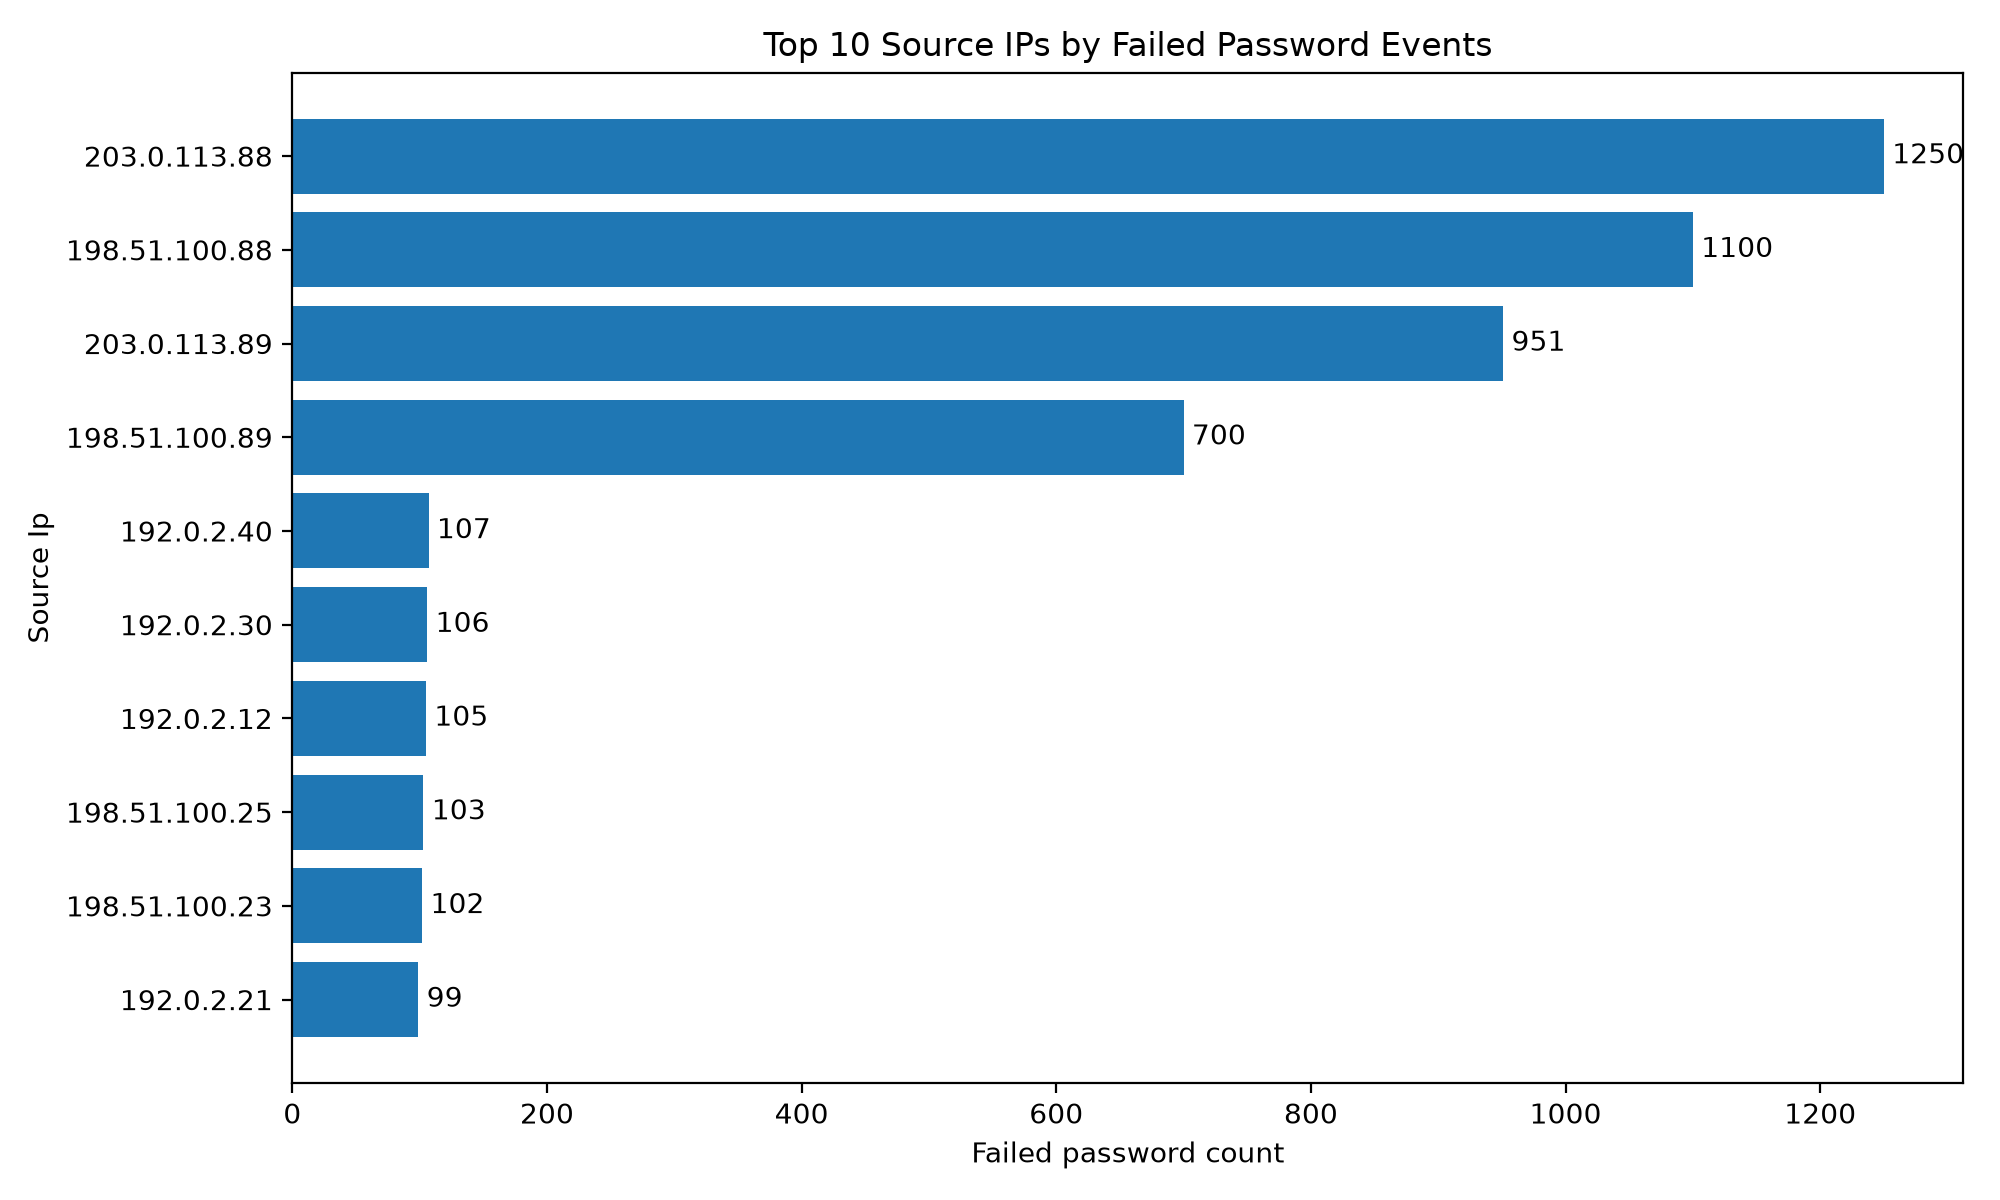
\includegraphics[width=0.76\linewidth]{output/top_source_ips_failed.png}
\caption{Top source IPs by failed password attempts. Four sources dominate SSH failure volume; \texttt{203.0.113.89} is notable because it later records a successful \texttt{backup} login.}
\end{figure}

The failed passwords point to SSH credential guessing across many accounts. Four sources account for 4,001 of 5,176 failures (77.3\%): \texttt{203.0.113.88}, \texttt{198.51.100.88}, \texttt{203.0.113.89}, and \texttt{198.51.100.89}; full counts are in Appendix~\ref{app:evidence-risk}, Table~\ref{tab:app-source-ips}. The generic usernames targeted (\texttt{root}, \texttt{admin}, \texttt{deploy}, \texttt{postgres}, \texttt{oracle}), together with the multi-account pattern, are consistent with automated, opportunistic SSH scanning rather than a campaign tailored to this organisation. On its own this activity is background noise, not evidence of compromise. \texttt{203.0.113.89} matters because it crosses from repeated failure to accepted access to the service account.

\tightsection{4. Attacker Lifecycle: The \texttt{203.0.113.89} Sequence}

\begin{figure}[H]
\centering
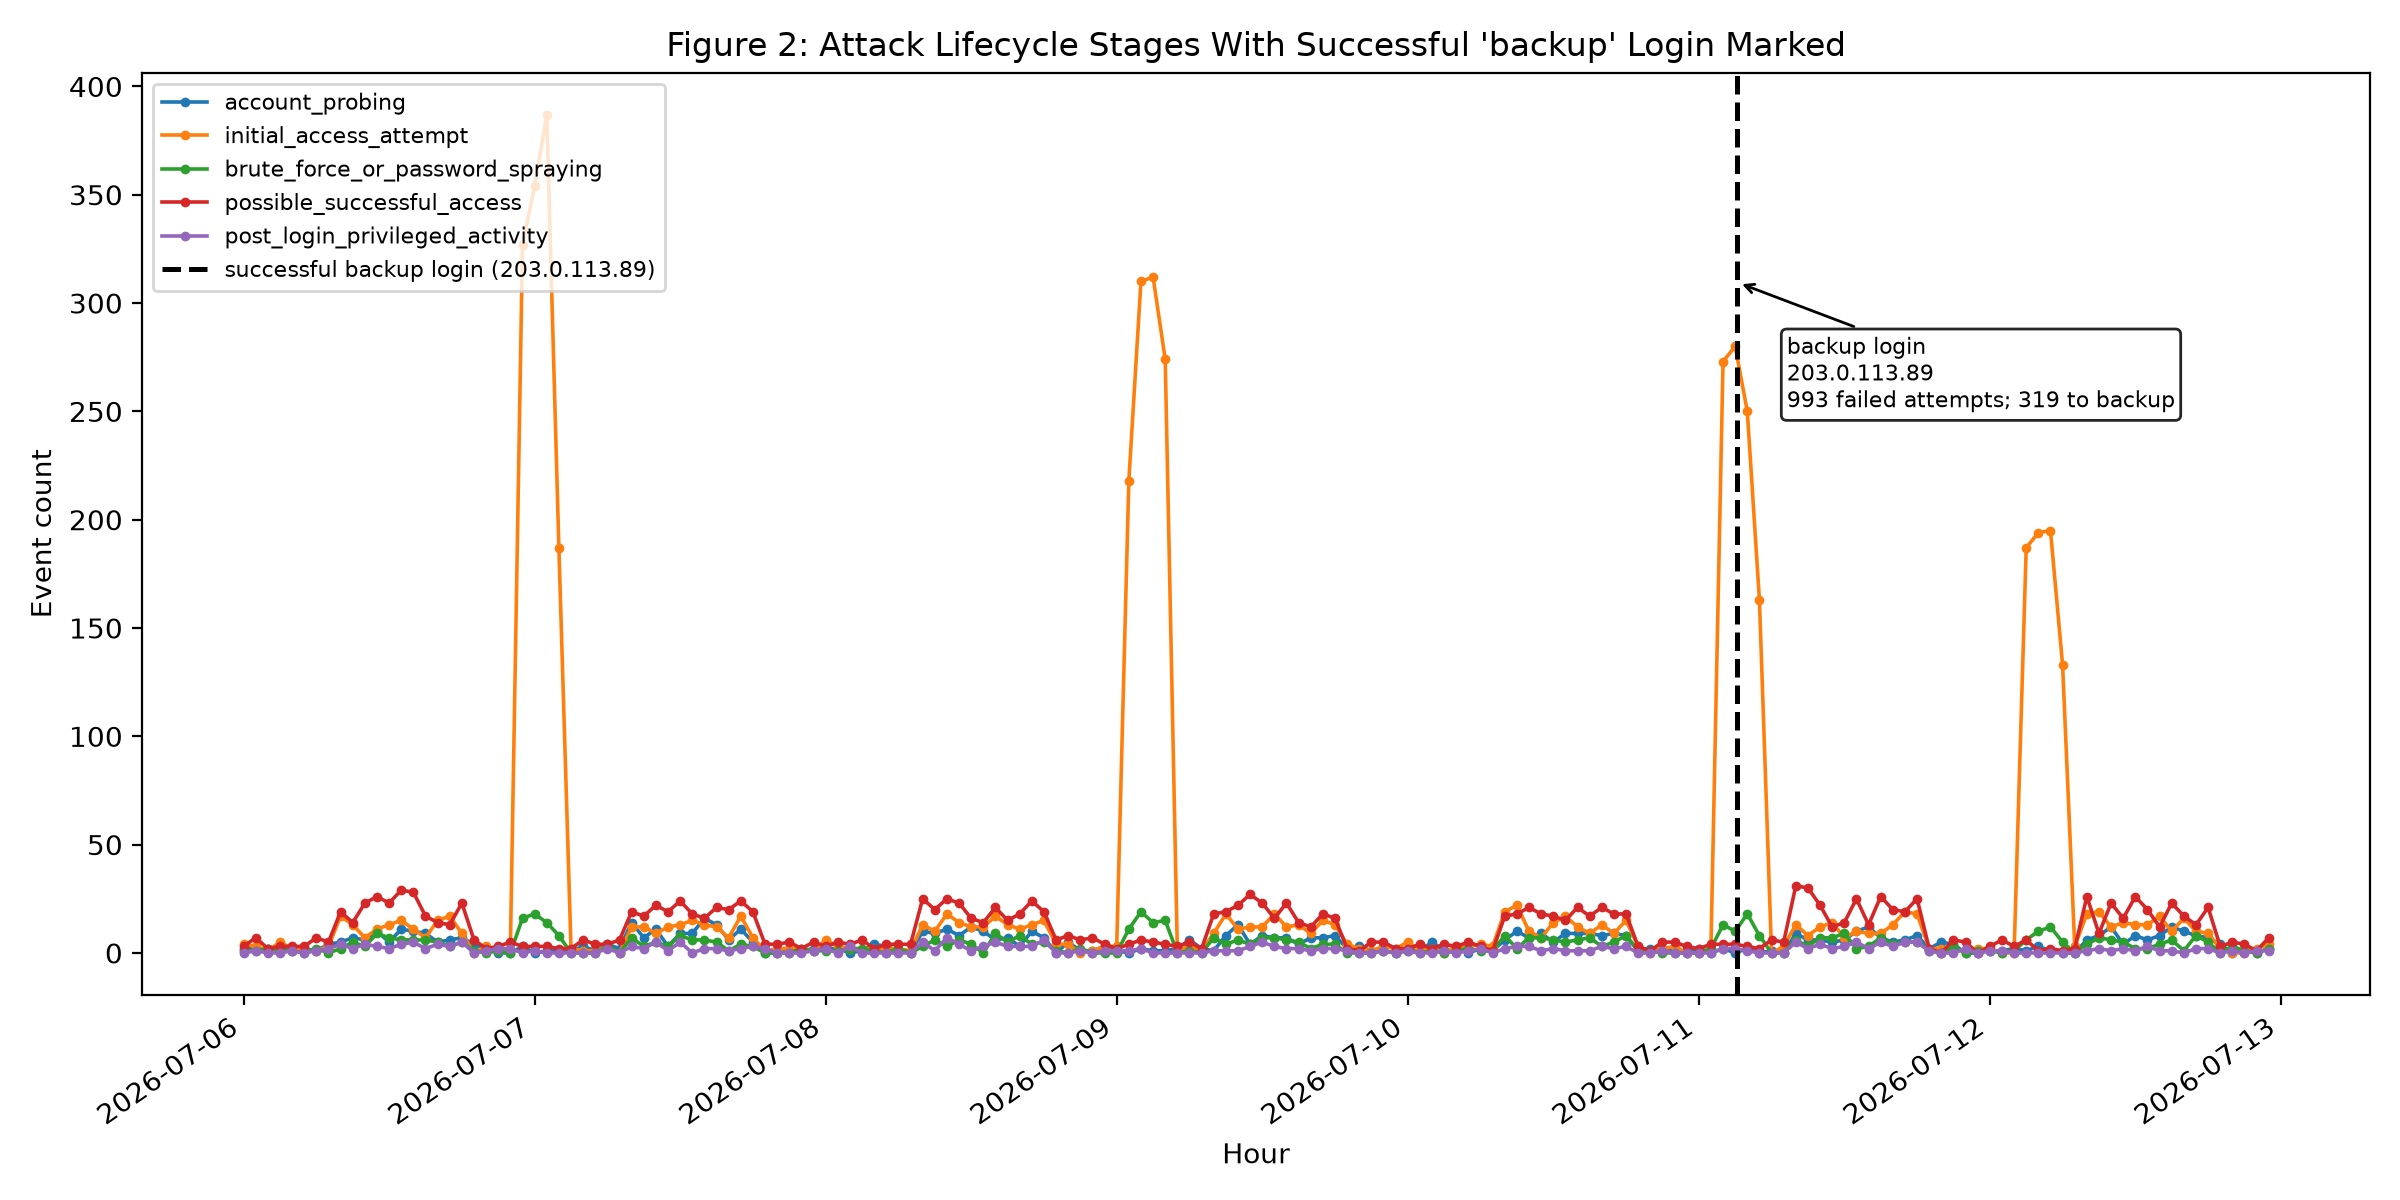
\includegraphics[width=0.86\linewidth]{output/figure2_attack_stages_backup_login.png}
\caption{Attack lifecycle stages over time with the successful \texttt{backup} login marked. The successful login occurs during an initial-access spike on Jul 11.}
\end{figure}

The key finding is an outlying failure-to-success sequence from one source on Jul 11. In the 60 minutes before acceptance, \texttt{203.0.113.89} generated 87 failed passwords against \texttt{backup}; across the other 389 accepted \texttt{backup} logins, no source exceeded three account-specific failures in the preceding hour. The source had no earlier accepted \texttt{backup} login in the extract. It then recorded an accepted login, same-user session activity, and root-level sudo commands. Scanning continued after acceptance, which is consistent with an automated attack wave rather than proof that every event from the address belonged to one interactive operator.

\begin{table}[H]
\centering
\caption{Critical Jul 11 authentication-to-sudo evidence chain.}
\footnotesize
\begin{tabularx}{\linewidth}{L{1.2cm}Y L{3.0cm}}
\toprule
Time & Evidence and interpretation & ATT\&CK \\
\midrule
03:07:30 & Failed login for invalid user \texttt{oracle} from \texttt{203.0.113.89}; account probing. & T1110.001; consistent with T1087 \\
03:07:32 & Failed password for \texttt{root} from \texttt{203.0.113.89}; privileged-account targeting. & T1110.001 \\
03:08:19 & Accepted password for \texttt{backup} from \texttt{203.0.113.89}; valid-account access over SSH. & T1078; T1021.004 \\
03:08:19 & \texttt{pam\_unix(sshd:session)} opened for user \texttt{backup}; session establishment. & T1021.004 \\
03:08:19 & \texttt{backup} runs \texttt{journalctl -n 200} and \texttt{systemctl status cron} as root; privileged post-login activity. & T1548.003 \\
\bottomrule
\end{tabularx}
\end{table}

The sequence maps most cleanly to T1110.001 $\rightarrow$ T1078 $\rightarrow$ T1021.004 $\rightarrow$ T1548.003: password guessing reaches a valid account over SSH, whose sudo rights expose a path to root. The two exact commands, \texttt{journalctl -n 200} and \texttt{systemctl status cron}, occur only at this timestamp, but related journal and service-status commands are common in legitimate sessions. They therefore support possible privileged reconnaissance, not confirmed malicious action. Same-second timing is not itself anomalous: all 255 sudo events in the extract have a same-second accepted-login match. Syslog's one-second precision and the different SSH process IDs also prevent a definitive session-level linkage. The stronger evidence is the account-specific failure baseline, source novelty, accepted login, and same-user privileged activity considered together. A short raw excerpt is in Appendix~\ref{app:raw-excerpt}.

\textbf{Temporal pattern.} Brute-force activity is concentrated outside working hours: roughly 70\% of failed logins (3,643 of 5,176) fall between 00:00 and 05:59, with a further spike around 23:00. Accepted logins cluster in business hours (08:00--18:00). For \texttt{backup} specifically, only 27 of 390 accepted logins (6.9\%) occur from 00:00 to 05:59, so 03:08 is uncommon but not outside the observed account baseline. Time of day strengthens the failure-to-success finding but cannot establish unauthorised use by itself (see Appendix~\ref{app:evidence-risk}, Table~\ref{tab:app-time-window}). Host-local time is assumed because no timezone is recorded.

\tightsection{5. Risk Prioritisation}

Asset: \texttt{backup01}, including its assumed production backup data, SSH access surface, \texttt{backup} service account, and sudo-to-root path. Its organisational value is not only the stored data but also its ability to restore production after failure or attack. The three prioritised risks trace the observed path from unauthorised access, through host control, to loss of backup confidentiality, integrity, availability, and recovery capability. The full matrix is included in Appendix~\ref{app:evidence-risk}, Table~\ref{tab:app-risk-matrix}.

R1 is the top priority because the source moves beyond attempted access: it is the only high-volume source that obtains an accepted login, after an account-specific preceding-hour pattern far outside the established-source baseline. The account's access to production backups and root-capable sudo path increase the potential consequence. Secondary risks, including SSH-service degradation and exposure of other sudo-capable accounts, remain relevant but are not prioritised here. Figure~\ref{fig:app-targeted-users} also shows that \texttt{backup} received the highest number of failed-password and maximum-authentication events among extracted usernames.

\tightsection{6. Initial Response and Investigation Limitations}
Immediate response should verify whether the \texttt{backup} login from \texttt{203.0.113.89} was authorised, rotate or disable the \texttt{backup} credentials until confirmed, preserve relevant logs, and review sudo, cron, journal, shell history, and audit evidence. High-volume SSH sources should also be blocked or rate-limited.

This evidence is limited to \texttt{auth.log}. It shows authentication, session, and sudo activity, but not every shell command, the network path to SSH, or whether firewall filtering was present. Timestamp-order examples in Appendix~\ref{app:evidence-risk}, Table~\ref{tab:app-timestamp-anomalies} are evidence limitations, not proof of tampering. Therefore, the extract supports likely brute-force activity, possible successful credential compromise, and privileged reconnaissance, but it does not prove public Internet exposure, botnet activity, malware execution, persistence, exfiltration, log deletion, or destructive tampering. The IP ranges are documentation-style ranges, so no real-world attribution or geolocation should be inferred.
